\chapter{Cyclone V SoC-FPGA}\label{cap:soc}

% Definição simples de SoC, dois ou três parágrafos e uma imagem
%================================
SoC é um acrônimo de System-on-a-Chip ou apenas System on Chip, como o nome já indica, um SoC é um sistema computacional inteiro contido em apenas um circuito integrado. Sendo assim, um SoC pode combinar diferentes elementos, em diferentes configurações, para formar um sistema completo.  Portando um SoC não se restringe à apenas um processador, além da CPU,  ele integra memória, periféricos de controle, como por exemplo, barramento de comunicação USB, unidade de processamento gráfico, e outros periféricos específicos para uma determinada aplicação.  

Para \citeonline{MichelSoC}, um system-on-chip é uma arquitetura que estabelece uma montagem de processadores, memórias, e interconexões feitos sobre medida para uma determinada aplicação. A figura~\ref{fig:socbasic} ilustra um SoC com alguns elementos básicos, que pode incluir múltiplos processadores  de diferentes arquiteturas, interconectados com uma ou mais memórias, isso pode oferecer meios de se criar sistemas reconfiguráveis, adicionando maior flexibilidade a um SoC.  Em muitas ocasiões um SoC pode ser equipado com componentes analógicos, como conversores analógicos digitais.


\begin{figure}[ht]
	\caption{Esquema SoC básico}
	\begin{center}
		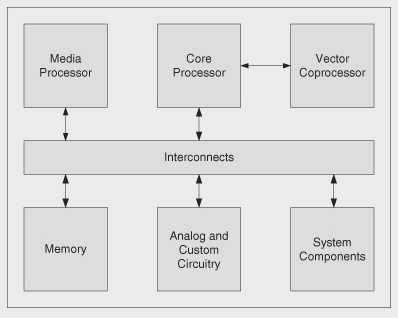
\includegraphics[scale=0.68]{imagens/basicsoc.png}\\
		{\small \textbf{Fonte:} \citeonline{MichelSoC}}
    \end{center}\label{fig:socbasic}
\end{figure}

% Descrição Cyclone V pincipais característica, famílias, imagem 
%================================

Dentre os dispositivos classificados como SoC, a Intel fornece uma linha de produtos classificados como SoC-FPGA, estes dispositivos se caracterizam por possuir um rede de FPGA integrados a um Processador ARM\@. Uma família de produtos que possuem essa característica é a Cyclone V SoC-FPGA\@. Estes componentes são constituídos por um Hardware Processor System que possui processadores ARM Cortex-A9 de um ou dois núcleos e um FPGA\@. A Figura~\ref{fig:socfpga} oferece uma visão global da integração entre os dois componetes principais do SoC-FPGA da família Cyclone V. 

\begin{figure}[ht]
	\caption{Diagrama de blocos simplificado Cyclone V}
	\begin{center}
		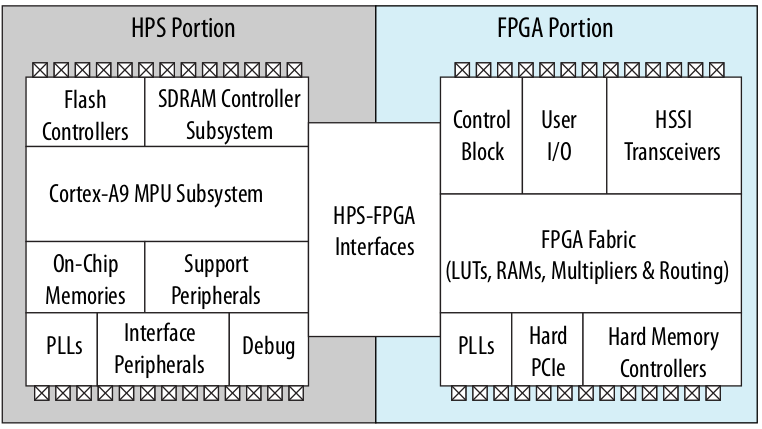
\includegraphics[scale=0.46]{imagens/socfpga.png}\\
		{\small \textbf{Fonte:} \citeonline{alteraCV}}
    \end{center}\label{fig:socfpga}
\end{figure}

Lançada iniciante pela Altera que foi adquirida em 2015 pela Intel~\cite{intelbuyaltera}, a família Cyclone V SoC-FPGA alia o poder de processamento do processador Cortex-A9 à versatilidade e flexibilidade do FPGA, o que faz desta linha de componentes possuirem um alto poder de processamento aliado a um baixo consumo. Os caminhos de interconexão entre o HPS e o FPGA do Cyclone V proporciona altas taxas de transferência, o que seria inviável em sistemas com dois chips. Esta estratégia de integração em um único circuito integrado oferece~\cite{CycloneV}:

\begin{itemize}
    \item Largura de banda de pico de mais de 100 Gbps.
    \item Coerência de dados integrada.
    \item Significativa economia de energia do sistema, eliminando caminhos de E/S externos entre o processador e o FPGA\@.
\end{itemize}

Este nível de integração entre os dois componentes que formam o SoC FPGA, provê um sistema com baixa potência dissipada, aliado a um reduzido custo e  espaço da placa necessária para a montagem do sistema. Ou seja o uso dos SoC-FPGA, com processador ARM combinado com FPGA, interligados através de um backbone de alta largura de banda e baixa potência, disponíveis nos produtos da linha da família Cyclone V da Intel, possibilita o desenvolvimento de aplicações com excelente desempenho, alta flexibilidade, além de baixo custo e baixo consumo de energia. 

\section{ARM Cortex-A9}
O processador Cortex A9 é uma linha de processadores ARM otimizados para alcançarem maior desempenho aliado a um baixo consumo. Esta linha de processadores ARM é uma das mais utilizadas, nas mais diversas aplicações, fazendo com que o ARM Cortex A9 seja um processador confiável e robusto. O Cortex A9 possui uma estrutura interna configurável, o que oferece flexibilidade ideal para o desenvolvimento de um novo SoC.  Na Tabela~\ref{tab:cortexA9config} são listadas algumas das configurações básicas do processador Cortex A9.

\begin{table}[ht]
    \caption{Estrutura típica de um pacote ROS }
    \begin{center}    
        \begin{tabular}{ll}
        \hline \hline
        Arquitetura                     & Armv7-A                                     \\ \hline \hline
        Multicore                       & 1-4 cores                                   \\ \hline \hline
        \multirow{7}{*}{Suporte ISA}    & Armv7-A                                     \\ \cline{2-2} 
                                        & Thumb-2 or Thumb                            \\ \cline{2-2}
                                        & TrustZone security technology               \\ \cline{2-2}
                                        & Jazelle DBX and RCT technologies            \\ \cline{2-2}
                                        & DSP extention                               \\ \cline{2-2}
                                        & Neon (Opcional)                             \\ \cline{2-2}
                                        & Floating Point (Opcional)                   \\ \hline \hline
        Memory Management Unit (MMU)    & Armv7 Memory Management Unit                \\ \hline \hline
        Debug and Trace                 & CoreSight                                   \\ \hline \hline
        \multirow{4}{*}{Characteristics}& Dual-issue, partially out-of-order pipeline \\ \cline{2-2}
                                        & \begin{tabular}[c]{@{}l@{}}Arquitetura do sistema flexível com
                                            \\caches configuráveis\end{tabular}       \\ \cline{2-2}
                                        & System coherency com ACP port               \\ \cline{2-2}
                                        & \begin{tabular}[c]{@{}l@{}}Desempenho 50\% maior do que  
                                            \\ o processador Cortex-A8  configurado 
                                            \\ como single-core\end{tabular}          \\ \hline\hline
        \end{tabular}
        \\{\small \textbf{Fonte:} \citeonline{armCortexA9}}
    \end{center}\label{tab:cortexA9config}
\end{table}

\subsection{Cortex-A9 MPCore Processor}
O Cortex-A9 MPCore processor é formado por três partes. Estas partes são componentes configuráveis que proporcionam a flexibilidade necessária para implementação de sistemas dedicados sobre medida para determinada aplicação. Os componentes do Cortex-A9 MPCore são \cite{mpcore}:

\begin{itemize}
    \item De um a quatro processadores Cortex-A9, que podem ser agrupados em um cluster, e um Snoop Control Unit (SCU) que pode ser usado para assegurar a coerência do cluster.

    \item Um conjunto de periféricos de memória mapeada, incluindo timer global, watchdog e timer privativo para cada processador contido no cluster
    
    \item Um controlador de interrupção integrado que é uma implementação do Generic Interrupt Controller. 
\end{itemize}

É possível implementar apenas um processador no cluster do Cortex-A9 MPCore, para isso, o processador deve ser implementado com suas próprias configurações de hardware. Mesmo contendo apenas um processador un SCU ainda estaré disponível, bem como ACP como um opcional. A Figura~\ref{fig:mpcore} apresenta um diagrama que representa o Cortex-A9 MPCore processor.

\begin{figure}[ht]
	\caption{Cortex-A9 MPCore Processor}
	\begin{center}
		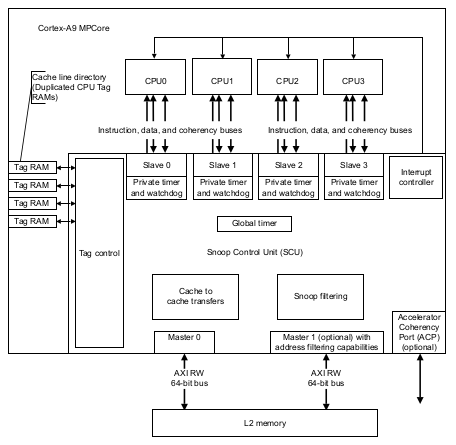
\includegraphics[scale=0.76]{imagens/mpcoreA9.png}\\
		{\small \textbf{Fonte:} \citeonline{mpcore}}
    \end{center}\label{fig:mpcore}
\end{figure}

% \subsection{Protocolo AMBA 3}
% \subsection{Generic Interrupt Control - GIC}

\section{Field Programmable Gate Array - FPGA}


\section{Hardware Processos System}
% Introdução, comentar sobre a família de processadores arm
%%================================
\subsection{FPGA Manager}
\subsection{HPS-FPGA Manager}
\subsection{HPS-FPGA Bridge}
\subsection{System Interconnect}
\subsection{Cortex-A9 Microprocessor Unit Subsystem}
ARM processors are the standard in embedded systems. Altera SoC FPGAs leverage one of ARM's latest, high-performance Cortex-A9 processor architectures.
\subsection{DMA Controller }
\subsection{Booting}


\section{Kit de desenvolvimento DE10-nano}